\documentclass[12pt,a4paper]{article} % Add twocolumn for two-column layout

% Packages
\usepackage[utf8]{inputenc} % UTF-8 encoding
\usepackage[T1]{fontenc}    % Better font encoding
\usepackage{geometry}       % Page layout
\geometry{a4paper, margin=1in}
%% \usepackage{graphicx}       % For images
\usepackage{subcaption}
\usepackage{amsmath, amssymb} % Math symbols
\usepackage{hyperref}       % Hyperlinks
\usepackage{xcolor}         % Text coloring
\usepackage{enumitem}       % Custom lists
\usepackage{caption}        % Captions for figures and tables
\usepackage{booktabs}       % Nicer tables
\usepackage{fancyhdr}       % Custom headers and footers
\usepackage{titlesec}       % Custom section formatting
\usepackage{multicol}       % Multicolumn support
\usepackage{csvsimple}      % Table support
\usepackage{pgfplotstable}
\usepackage{rotating}       % For rotating the table
\usepackage{listings}       % Code blocks
\usepackage{indentfirst}
\usepackage{float}



%% \usepackage{showframe}     % Debug

% Custom Header/Footer
\pagestyle{fancy}
\fancyhf{}
\fancyhead[C]{BI-PST Homework}
\fancyfoot[C]{\thepage}

\newcommand{\randv}[2][X]{#1_{\text{#2}}}
\newcommand{\E}{\mathbb{E}}
\newcommand{\var}{\text{var}}

% Section Formatting
\titleformat{\section}{\large\bfseries}{\thesection}{1em}{}
\titleformat{\subsection}{\normalsize\bfseries}{\thesubsection}{1em}{}

% Title Information
\title{BI-PST/24-25 Homework}
\author{Oleksandr Slyvka\\ slyvkole@cvut.cz  \and Illia Lyhin  \\ lyhinill@cvut.cz \and Maksym Khavil \\ khavimak@cvut.cz }
\date{\today} % Can replace with a fixed date or leave blank

\pgfplotstableread[col sep=comma]{./data/case0202.csv}\datatable

\begin{document}
% Title Page
\maketitle
\begin{abstract}
With this document we present homework for BI-PST. Oleksandr Slyvka was chosen as a represntative for our group. He was born 14.04.2006, so we get $K=14$ and $L=6$, then $M = 4$. Such value of $M$ corresponds to case0202 Sleuth dataset, volume of hippocampus with respect to schizofrenia. We will analyse this dataset using numpy, pandas, matplotlib and scipy.stats Python modules.
\end{abstract}
\vspace{1em}

% Sections
\section{Data and estimating moments}

\begin{multicols}{2}

  Firstly, we will load data and display it as a table. There are $n=15$ samples in both categories, values seem to be greater than $1 \text{cm}^3$ and peak around $2 \text{cm}^3$, each row repesents a pair of twins, one of whom was affected by schizophrenia and other was not.
\columnbreak

\pgfplotstableread[col sep=comma]{./data/case0202.csv}\datatable

  \csvautotabular{./data/case0202.csv} % Auto-generates a table from the CSV
%  \caption{case0202}
%  \label{tab:case0202}

\end{multicols}
\pagebreak

\subsection{Estimations}
  Let $\randv{unaff}$ and $\randv{aff}$ denote random variables of hippocampues volume of those who are unaffected and affected by schizofrenia respectively, we will refer to them as unaffected and affected distributions or random variables. We will compute estimates of mean, median and variance of those random variables. Median estimation will be chosen as 7th value of sorted sequence of data points also known as midpoint. Estimated mean and variance will be computed with following formulas:

\begin{align*}
  \widehat{\E\randv{}} &= m_1 = \bar{X} = \frac{1}{n} \sum_{k = 1}^{n}X_i\\
  \widehat{\var\randv{}} &= s^2 = \frac{1}{n - 1} \sum_{k = 1}^n(X_i - \bar{X})^2
\end{align*}

  Additionaly we will compute uncorrected biased variance.

\begin{equation*}
  S^2 = \frac{1}{n} \sum_{k = 1}^n(X_i - \bar{X})^2
\end{equation*}

  All those computations are done by the following code:

\begin{lstlisting}[basicstyle=\scriptsize]
    print(f'{'Mean:' :<30}{X.mean():.3f}')
    print(f'{'Median:' :<30}{X.median():.3f}')
    print(f'{'Variance without correction:' :<30}{((X - X.mean()) ** 2).sum() / n :.3f}')
    print(f'{'Variance with correction:' :<30}{((X - X.mean()) ** 2).sum() / (n - 1):.3f}')
\end{lstlisting}

  After plugging values in, we obtain such results.

\begin{align*}
  \widehat{\E\randv{unaff}} &= 1.759 & \widehat{\E\randv{aff}} &= 1.560 \\
  \widehat{F^{-1}_{\randv{unaff}}(0.5)} &= 1.770 & \widehat{F^{-1}_{\randv{aff}}(0.5)} &= 1.590 \\
  \widehat{\var\randv{unaff}} &= 0.059 & \widehat{\var\randv{aff}} &= 0.091 \\
  S^2_{\text{unaff}} &= 0.055 & S^2_{\text{aff}} &= 0.085
\end{align*}

Let's notice that estimated expected value of unaffected distribution is greater than estimated expected value of affected distribution.

\pagebreak
\section{Histograms and empirical cumulitive distribution functions}

We will plot histograms, width of bins will be $0.2 \text{cm}^3$. By their side we will plot empirical cumulitive distribution functions, they will have a step of $1/n$ at each sample value.

Let's plot histogram and ecdf for distribution of unaffected twins.

\begin{figure}[h]
  \centering
  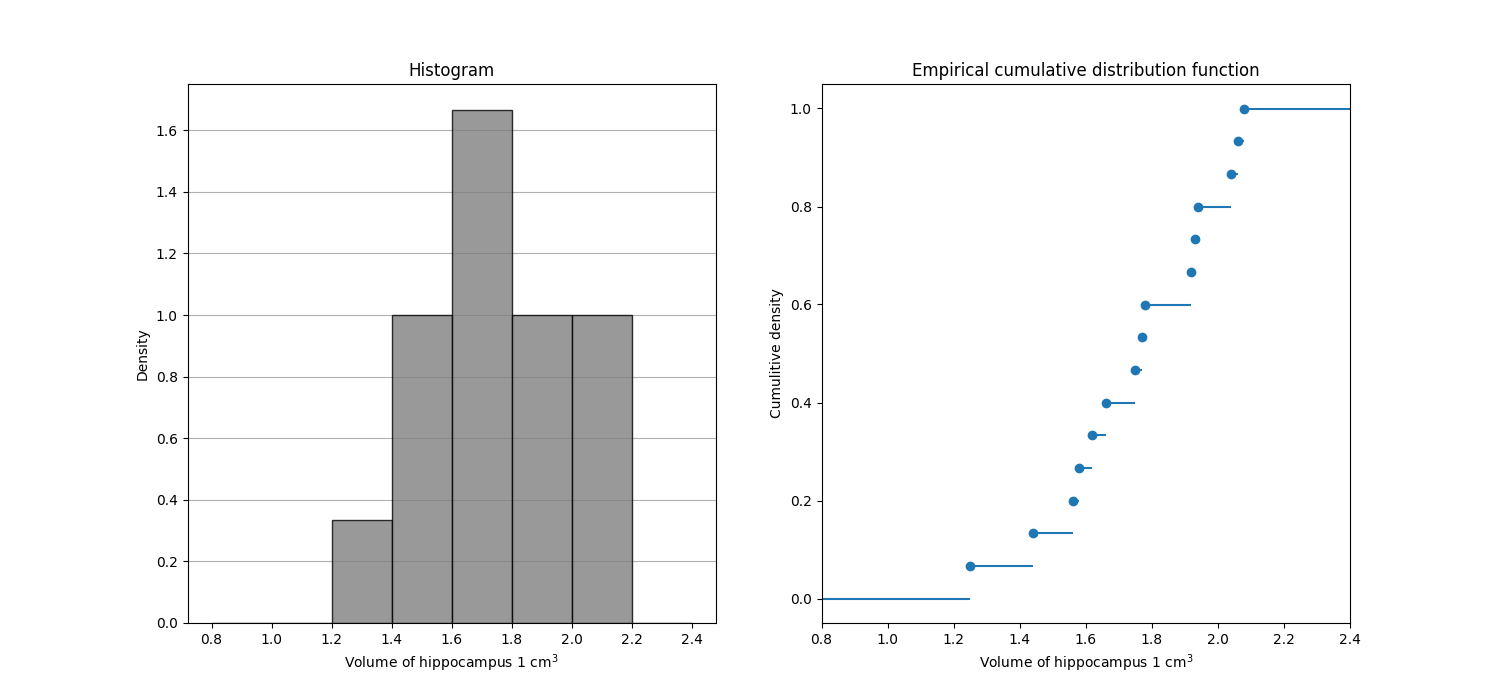
\includegraphics[scale=0.4]{./img/unaffected_hist_ecdf.png}
  \label{fig:unaff_ecdf}
  \caption{Unaffected distribution}
\end{figure}

Here is the same plot for distibution of schizophrenic twins.
\begin{figure}[h]
  \centering
  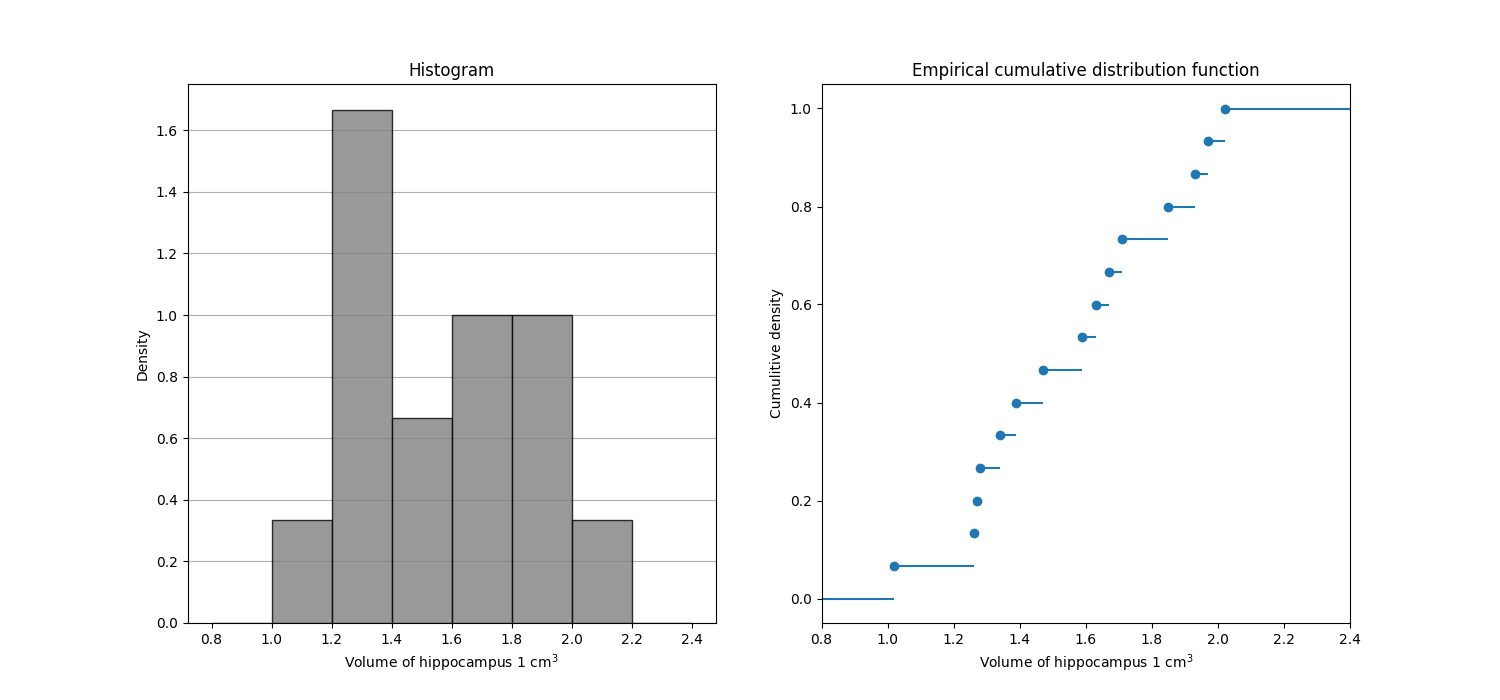
\includegraphics[scale=0.4]{./img/affected_hist_ecdf.png}
  \label{fig:aff_ecdf}
  \caption{Affected distribution}
\end{figure}

We can see that later histogram is a little wider, that corresponds with its variance being greater than variance of unaffected distributions. Another observation is that it is altogether slightly shifted towards zero.

\section{Choosing between normal, uniform and exponential distributions}

We will try to choose distribution for our data that will match it the best. To do that we need to find parameters of distributions, we will calculate them using method of moments. % TODO: insert link to original paper discussing MoM

\subsection{Calculating parameters}

Normal distribution is parametrized by $\mu$ and $\sigma^2$, uniform distribution is parametrized by its lower and upper bounds resp. $a$ and $b$ and exponential one is parametrized by the rate $\lambda$. All of them can be expressed as functions of at least two moments (exponential can be derived using single moment). Exception will be variance, as method of moments yields biased estimation, so we will use Bessel corrected estimation.

\begin{align*}
  \hat \mu &= m_1 \\
  \hat \sigma^2 &= \frac{n}{n - 1} \cdot (m_2 - m_1^2) \\
  \hat a &= m_1 - \sqrt{3(m_2 - m_1^2)}\\ 
  \hat b &= m_1 + \sqrt{3(m_2 - m_1^2)}\\ 
  \hat \lambda &= \frac{1}{m_1}
\end{align*}

Those computations are calculated in this code:

\begin{lstlisting}
    m1 = X.mean()
    m2 = (X ** 2).mean()
    mu_hat= m1
    sigma2_hat=  (n / (n - 1))* (m2 - m1 ** 2)
    lambda_hat = 1 / m1
    a_hat = m1 - np.sqrt(3 * (m2 - m1**2))
    b_hat = m1 + np.sqrt(3 * (m2 - m1**2))
    print(f"Normal: {mu_hat=}, {sigma2_hat=}")
    print(f"Exp: {lambda_hat=}")
    print(f"Uniform: {a_hat=}, {b_hat=}")
\end{lstlisting}

After we have it run we get following values.

\begin{align*}
  &\text{Unaffected}       & &\text{Affected} \\
  &\hat\mu = 1.758         & &\hat\mu = 1.559\\
  &\hat\sigma^2 = 0.059    & &\hat\sigma^2 = 0.091\\
  &\hat a = 1.353          & &\hat a = 1.055\\
  &\hat b = 2.164          & &\hat b = 2.064\\
  &\hat\lambda = 0.568     & &\hat\lambda = 0.641\\
\end{align*}


\subsection{Comparing histogram and probability distribution functions}

\begin{figure}[H]
\centering
\begin{subfigure}{0.48\textwidth}
  \centering
  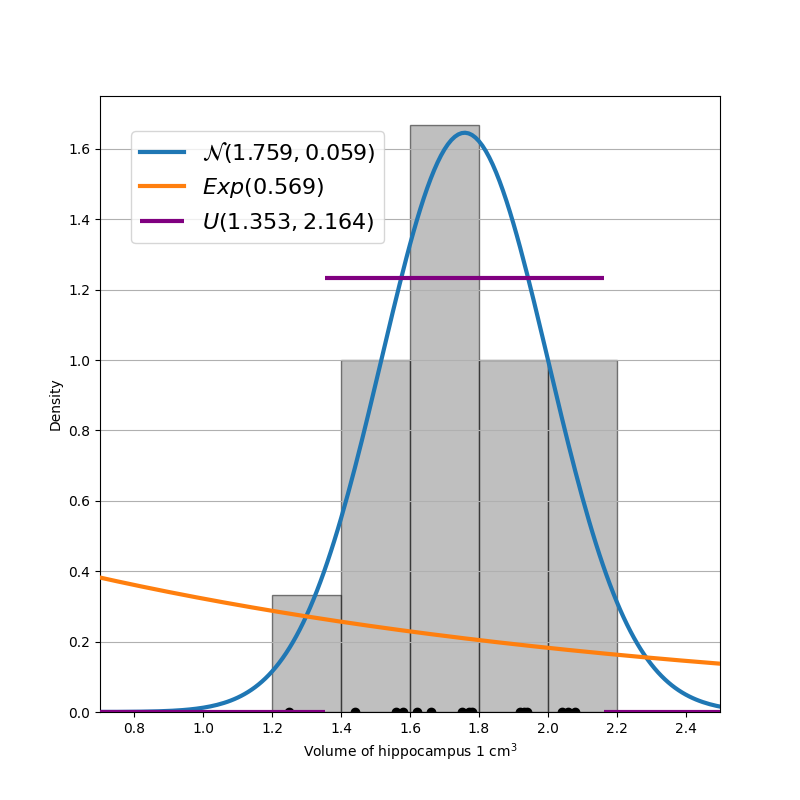
\includegraphics[scale=0.4]{./img/unaffected_distributions.png}
  \label{fig:unaff_dists}
  \caption{Unaffected}
\end{subfigure}
\begin{subfigure}{0.48\textwidth}
  \centering
  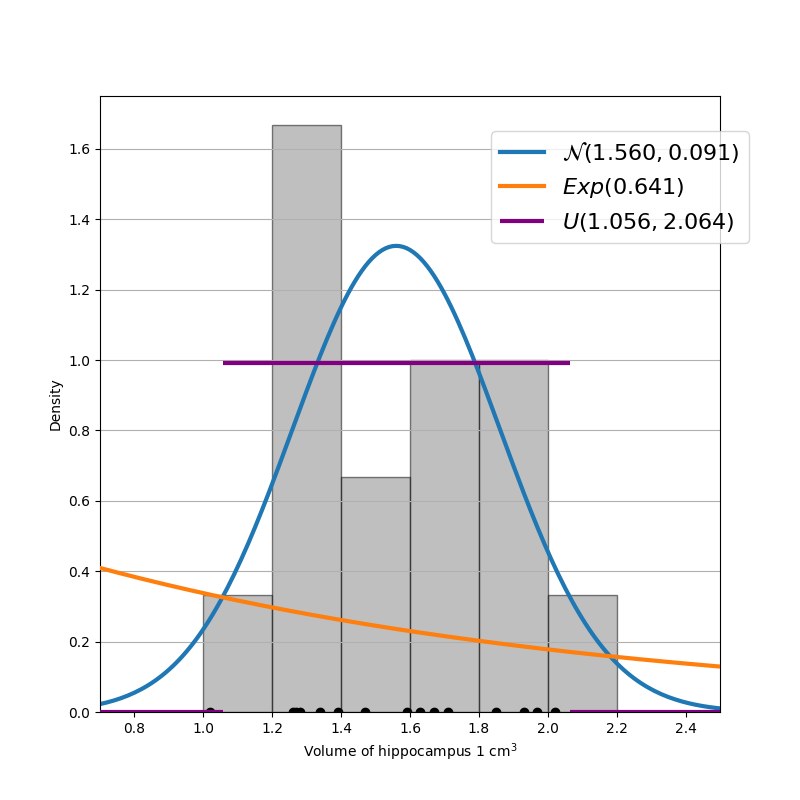
\includegraphics[scale=0.4]{./img/affected_distributions.png}
  \label{fig:aff_dists}
  \caption{Affected}
\end{subfigure}
  \caption{Histograms and pdfs}
\end{figure}

In both cases exponential distribution performs horribly, so we will reject it immideatly. At both plots there are data points (black dots on x-axis), that lay in zero-probability area for uniform distribution, so it will be rejected too. We are left only with normal distribution, so we naturally choose it, in addition it matches histogram peaks quite nicely.
\newpage

\section{Comparing histograms of 100 generated samples and data}

We have computed parameters $\hat\mu = 1.76$ and $\hat \sigma^2 = 0.05$ for distribution of those, who were not affected, and $\hat\mu = 1.56$ and $\hat\sigma^2 = 0.08$ for those who were. We will generate a 100 random samples using following code:

\begin{lstlisting}
samples = stats.norm.rvs(
    loc=mu_hat, scale=np.sqrt(sigma2_hat),
    size=100, random_state=42
)
\end{lstlisting}

Now let's plot histograms and compare them.

\begin{figure}[h]
  \centering
  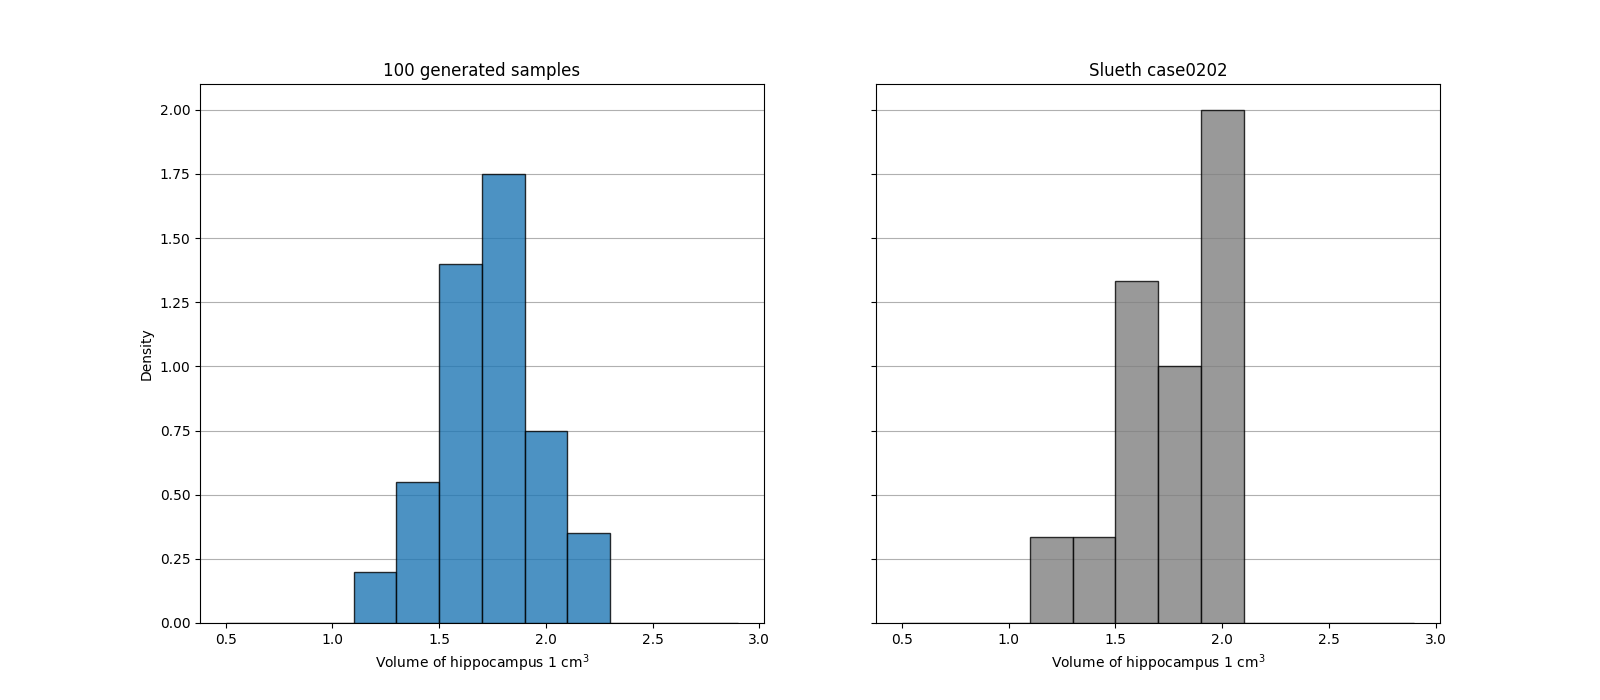
\includegraphics[width=\textwidth]{./img/comparing_generated_unaffected.png}
  \label{fig:comp_gen_unaff}
  \caption{Generated (left) and given (right) histograms of unaffected distributions}
\end{figure}

We can see that artificial one is more gravited towards mean, while given one is skewed right. Besides that they share number of similarities, their ranges match almost perfectly and they both have similar probabilities for peak and tail values.

\begin{figure}[H]
  \centering
  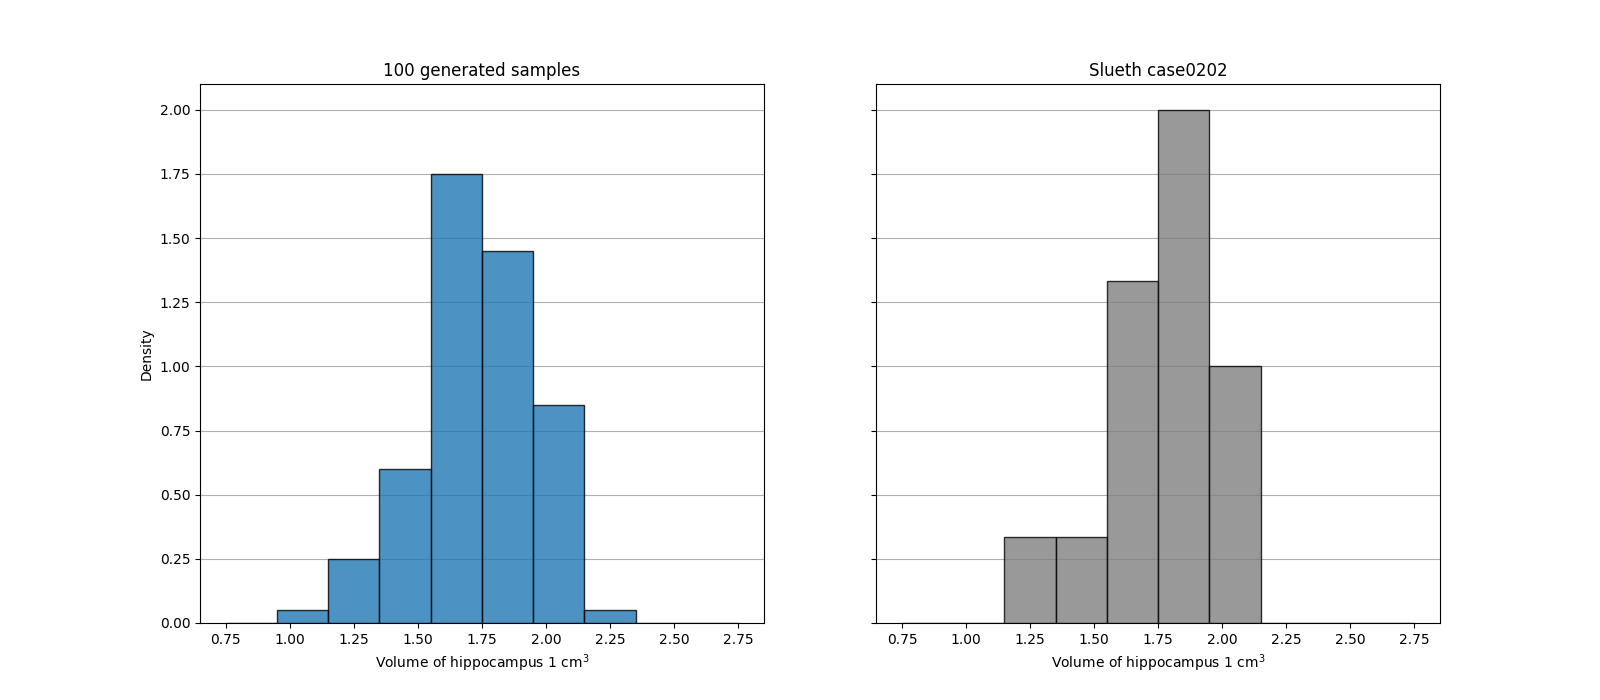
\includegraphics[width=\textwidth]{./img/comparing_generated_affected.png}
  \label{fig:comp_gen_aff}
  \caption{Generated (left) and given (right) histograms of affected distributions}
\end{figure}

Artificially generated histogram follows shape of data closely, though in this case it tends to be more spread out, with it peak sitting $0.4$ points lower and samples reaching further from center.

\section{Computing two-sided confidence intervals for expected value at $95\%$ level}

We do not have theoretical variance, so we will need to use $t$ distribution to derive our intervals. 

From lectures we have formula $ \text{CI} = \left(\bar{X}_n - \frac{t_{n-1}\left(\frac{\alpha}{2}\right) \cdot s}{\sqrt{n}}, \bar{X}_n + \frac{t_{n-1}\left(\frac{\alpha}{2}\right) \cdot s}{\sqrt{n}}\right)$, we calulate it with next Python code:

\begin{lstlisting}
    m = X.mean()
    s = np.sqrt(((X - X.mean()) ** 2).sum() / (n - 1))
    t_alpha_2 = stats.t.isf(alpha/2, df=n-1)
    L = m - t_alpha_2 * s / np.sqrt(n)
    R = m + t_alpha_2 * s / np.sqrt(n)
    return L, R
\end{lstlisting}

As a result we obtain these confidence intervals at 95\% level for $\randv{unaff}$ and $\randv{aff}$:

\begin{align*}
  &\text{CI}_{\text{unaff}} = (1.6244, 1.8929) \\
  &\text{CI}_{\text{aff}} = (1.3931, 1.7268)
\end{align*}

\section{Testing two-sided hypothesis that expected values equal $K$ at $5\%$ level}

Let's formulate hypothesis for unaffected distribution. Null hypothesis will be that expected value of $\randv{unaff}$ equals $K = 14$. Hypothesis for affected distribution can be formulated analogically.

\begin{align*}
  H_0 &: \E\randv{unaff} = K \\
  H_A &: \E\randv{unaff} \neq K
\end{align*}

To test this hypothesis we would need two-sided confidence intervals for mean. Luckily they were already computed, so we can reject null hypothesis for both affected and unaffected cases, because $K = 14 \not\in (1.39, 1.73)$ and $K = 14 \not\in (1.62, 1.89)$.

\section{Testing if means of affected and unaffected distributionsare  equal at $5\%$ level}

It is clear that null hypothesis is that expected values are equal. We choose right-sided alternative hypothesis, because pooled mean of affected distribution is lower than pooled mean of unaffected, so it will be natural to asssume that schizofrenia shrinks one's hippocampus. We can formulate hypotheses following way.

\begin{align*}
  H_0 &: \E\randv{aff} = \E\randv{unaff}\\
  H_A &: \E\randv{aff} < \E\randv{unaff}
\end{align*}\label{Hypotheses}

We will conduct right $t$-test for null hypothesis. One of its assumptions is that variances of both distributions are equal, we do not know theoretical values.

\subsection{Variance equalness test at $5\%$ level}

Let's formulate hypotheses for variance test:

\begin{align*}
  H_0 &: \var\randv{aff} = \var\randv{unaff}\\
  H_A &: \var\randv{aff} \neq \var\randv{unaff}
\end{align*}

We will conduct Levene test at $5\%$ level, if variances of both distributions are equal. We will use scipy.stats implementation for that test:

\begin{lstlisting}
stats.levene(X_aff, X_una, center='mean')
\end{lstlisting}

Plugging values in we obtain $p$-value of $0.274$, it is greater than $0.05$, so we fail to reject null hypothesis (equalness of variances) at $5\%$ level and we can further assume, that variances of the distributions are equal. 

\subsection{Conducting $t$-test for means}

Now we will try to test hypotheses defined in the begining of section \ref{Hypotheses}. Once again we will use scipy's implementation to conduct test:

\begin{lstlisting}
stats.ttest_ind(X_aff, X_una, equal_var=True, alternative='less')
\end{lstlisting}

This code yields $p$-value of $0.028$, it is less than $0.05$, so we reject null hypothesis $\E\randv{aff} = \E\randv{unaff}$ in favor of the alternative at $5\%$ level.

\section{Conclusion}
We have conducted analysis of Sleuth case0202 dataset, derived estimates for moments and chose normal distribution for both random variables. Lastly, we computed confidence intervals for means and tested if their expected values are equal by two sample $t$-test.


% Bibliography (Optional)
\begin{thebibliography}{99}
\bibitem{example} BI-PST 24/25, lectures
\end{thebibliography}

\end{document}
